\documentclass[aspectratio=169,11pt]{beamer}

% Shared style (ib-tutorials.sty at the repo root).
\makeatletter\def\input@path{{./}{../}}\makeatother
\usepackage{ib-tutorials}

\usepackage[utf8]{inputenc}
\usepackage{amsmath,amssymb}
\usepackage{booktabs}
\usepackage{array}
\newcolumntype{L}[1]{>{\raggedright\arraybackslash}p{#1}}
\usepackage{graphicx}
\graphicspath{{../pictures/5-visit/}{pictures/5-visit/}}
\usepackage{xcolor}
\usepackage{listings}
\usepackage{tikz}
\usetikzlibrary{arrows.meta,positioning,shapes.geometric,fit,calc}
\usepackage{hyperref}

\newcommand{\sourcecredit}[1]{\vfill\begin{flushright}\tiny\textcolor{DarkGray}{#1}\end{flushright}}
\newcommand{\gui}[1]{\textsf{\textbf{#1}}}

\lstset{
  basicstyle=\ttfamily\scriptsize\color{BlackGray},
  keywordstyle=\color{NavyBlue}\bfseries,
  commentstyle=\color{DarkGray}\itshape,
  stringstyle=\color{OliveGreen},
  showstringspaces=false,
  columns=fullflexible,
  keepspaces=true,
  breaklines=true,
  breakindent=1em,
  frame=single,
  framerule=0.4pt,
  rulecolor=\color{LightGray},
  backgroundcolor=\color{LightGray!30},
  xleftmargin=0.25em,
  xrightmargin=0.25em
}
\lstdefinestyle{shell}{morecomment=[l]{\#}}
\lstdefinestyle{python}{morecomment=[l]{\#}}
\lstdefinestyle{tiny}{basicstyle=\ttfamily\tiny\color{BlackGray}}
\lstdefinestyle{pytiny}{morecomment=[l]{\#},basicstyle=\ttfamily\tiny\color{BlackGray}}

\title[VisIt: movies]{VisIt: making movies}
\subtitle{Frames first, then one encoding command: the Save movie wizard, \texttt{visit -movie} with a session or a script, a loop of your own, and ffmpeg; fixed colour limits, a time stamp, the frame rate you asked for, and files that play everywhere}
\author[Miller]{Laura A. Miller}
\institute[UArizona]{Department of Mathematics, University of Arizona}
\date{Using IB Software \textbullet\ Part V \textbullet\ Chapter 30}

\begin{document}

% 1
\begin{frame}[plain]
\maketutorialtitlepanel{%
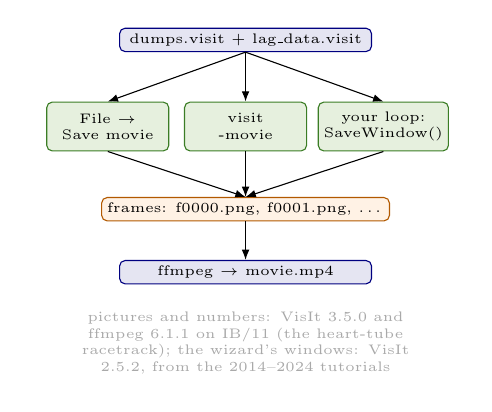
\begin{tikzpicture}[every node/.style={font=\tiny}, box/.style={draw, rounded corners=2pt, align=center, inner sep=2pt}]
  \node[box,draw=NavyBlue,fill=NavyBlue!10,minimum width=3.2cm] (d) at (2.6,1.95) {\code{dumps.visit} + \code{lag\_data.visit}};
  \node[box,draw=OliveGreen,fill=OliveGreen!10,minimum width=1.55cm,minimum height=0.62cm] (w) at (0.85,0.85) {File $\to$\\Save movie};
  \node[box,draw=OliveGreen,fill=OliveGreen!10,minimum width=1.55cm,minimum height=0.62cm] (m) at (2.6,0.85) {\code{visit}\\\code{-movie}};
  \node[box,draw=OliveGreen,fill=OliveGreen!10,minimum width=1.55cm,minimum height=0.62cm] (l) at (4.35,0.85) {your loop:\\\code{SaveWindow()}};
  \node[box,draw=orange!70!black,fill=orange!10,minimum width=3.2cm] (f) at (2.6,-0.2) {frames: \code{f0000.png}, \code{f0001.png}, \dots};
  \node[box,draw=NavyBlue,fill=NavyBlue!10,minimum width=3.2cm] (e) at (2.6,-1.0) {\code{ffmpeg} $\to$ \code{movie.mp4}};
  \foreach \t in {w,m,l} {\draw[-{Latex[length=1.3mm]}] (d.south) -- (\t.north); \draw[-{Latex[length=1.3mm]}] (\t.south) -- (f.north);}
  \draw[-{Latex[length=1.3mm]}] (f) -- (e);
  \node[text=DarkGray,align=center,text width=5.3cm] at (2.6,-1.9) {pictures and numbers: VisIt 3.5.0 and ffmpeg 6.1.1 on IB/11 (the heart-tube racetrack); the wizard's windows: VisIt 2.5.2, from the 2014--2024 tutorials};
\end{tikzpicture}}
\end{frame}

% 2
\begin{frame}{Learning goals}
\label{fr:goals}
\footnotesize By the end of this chapter you should be able to:
\begin{itemize}
  \item Prepare a plot for a movie: fixed colour limits, a fixed view, one legend, a time stamp, no refinement-level lines.
  \item Make the frames three ways: the \gui{Save movie} wizard, \code{visit -movie} with a saved session or a script, and a loop of your own.
  \item Turn frames into an MP4 that plays in slides, browsers and phones with one ffmpeg command; make a GIF; put two runs side by side.
  \item Choose the frame rate and the dump interval for the movie you want.
  \item Recognise the silent failures: no frames written, a structure that stands still, a frame rate you did not ask for, a file that will not play.
\end{itemize}
\begin{punchbox}
\small A movie is a folder of frames and one encoding command. Keep the frames, and fix everything that must not change from frame to frame (limits, view, legend) before the first one.
\end{punchbox}
\end{frame}

% 3
\begin{frame}{Where this chapter comes from}
\label{fr:sources}
\scriptsize
\begin{itemize}
  \item \al{N. Battista's tutorial, ``Part III: Let's make groovy movies!''} (2014, for UNC's Kure and Killdevil; the 2018 MATH 769 version is ``Run your first IBAMR simulation''): the first walk-through from \code{lag\_data.visit} to a movie: \gui{File $\to$ Save Movie}, \gui{New simple movie}, \gui{MPEG Movie} and the right arrow, start, end, frame rate and stride, a folder and a title (``cleverly titled FIRST\_SIMULATION\_MOVIE''), an e-mail if you like, and ``Now, use currently allocated processors''.
  \item \al{``VISIT -- How to visualize IBAMR Data''} (2020, slides 21--23 and 31; again in the 2021 deck) and \al{the 2024 IB2d practical} (slides 25--27): the same wizard steps with the 2014 pictures (the practical stops there, with \gui{MPEG Movie}); then the 2020 and 2021 decks, like \al{``Lecture 9: Sampling, averaging, and analyzing data in Visit''} (2019, slide 26), say ``Save as mpeg is not the best option'': save PNG or JPEG images and ``Put the set of images back together as a movie using VirtualDub (free for PC) or Quicktime Pro''.
  \item \al{L. Waldrop's guide ``Data analysis in VisIt''} (MATH 769, 16 February 2015, VisIt 2.5.2; the same text in its 2017 version for IB2d), ``Make a Movie of the Simulation'': the wizard page by page, and ``VisIt makes OK mpeg movies, but if you are readying this movie for a presentation, it will be better quality if you output TIFF or PNG images and stitch them together in a video player like Quicktime Pro''.
  \item \al{``3B -- Analyzing your IBFE simulation''} (2018), slides 3--8: record the GUI in Python, add a loop that saves a picture at every time, and run it with \code{visit -cli -nowin -s} on the cluster.
\end{itemize}
Chapter 4b already makes an IB2d movie this way (the wizard with PNG, then an ffmpeg line); this chapter is the whole story. \al{New here:} frames + ffmpeg and \code{visit -movie}, which no deck taught; \code{visit -movie} (the wizard's own engine) and a loop of your own run on IB/11 in VisIt 3.5.0 (Linux, no window) with ffmpeg 6.1.1, with what each writes, how long it lasts and how big it is; the wizard's 3.5 pages read from the program itself (the wizard itself was not run); and three scripts, \code{examples/analysis/visit\_movie\_frames.py}, \code{make\_movie.py} and \code{movie\_clean.py}.
\end{frame}

% 4
\begin{frame}{What the old decks taught, and what changed}
\label{fr:old}
\scriptsize
\begin{tabular}{@{}L{0.34\textwidth}L{0.62\textwidth}@{}}
\toprule
then & now \\
\midrule
\gui{File $\to$ Save movie $\to$ MPEG movie} (2014--2024) & the wizard is still there in 3.5, and lists MP4 beside MPEG when it finds ffmpeg (VisIt's movie formats are made by ffmpeg); ask it for PNG images and encode them yourself (slide \ref{fr:routes}) \\
``Save as mpeg is not the best option'' (2019--2021) & measured: VisIt's MPEG is MPEG-1 at 24 frames/s (it asks ffmpeg for 18 Mbit/s; ours averages 2.6), 2.0 MB for our 51 frames; ffmpeg's H.264 MP4 of the same frames is 0.56 MB (slide \ref{fr:formats}) \\
the wizard's frame rate & VisIt copies frames to make 30 frames/s, then ffmpeg plays the copies at 25 (MP4) or writes 24 (MPEG): 10 comes out as 8.3 (slide \ref{fr:fps}) \\
VirtualDub (``free for PC'') or QuickTime Pro to join the images & ffmpeg: free, the same command on Linux, macOS, Windows and the cluster. QuickTime 7 Pro is a 32-bit program, which macOS 10.15 and later do not run (Apple ended its Windows version in 2016); VirtualDub is Windows-only, last released (1.10.4) in 2013 \\
the 2018 loop: ``Note we advance in time to skip t=0'' & start at dump 0, and step every time slider (slide \ref{fr:loop}) \\
the coloured boxes hidden with \gui{Hide/Show} & delete the Subset plot of the levels (slide \ref{fr:levels}) \\
Killdevil's VisIt 2.12.3 and Python 2 & VisIt 3.5's Python 3; Puma in chapter 31 \\
\bottomrule
\end{tabular}
\sourcecredit{The decks of the previous slide; measurements: \code{wsl/final/ch30\_movies*.sh}, \code{ch30\_mp4.sh}.}
\end{frame}

% 5
\begin{frame}{The example: IB/11's racetrack, 51 dumps}
\label{fr:example}
\centering
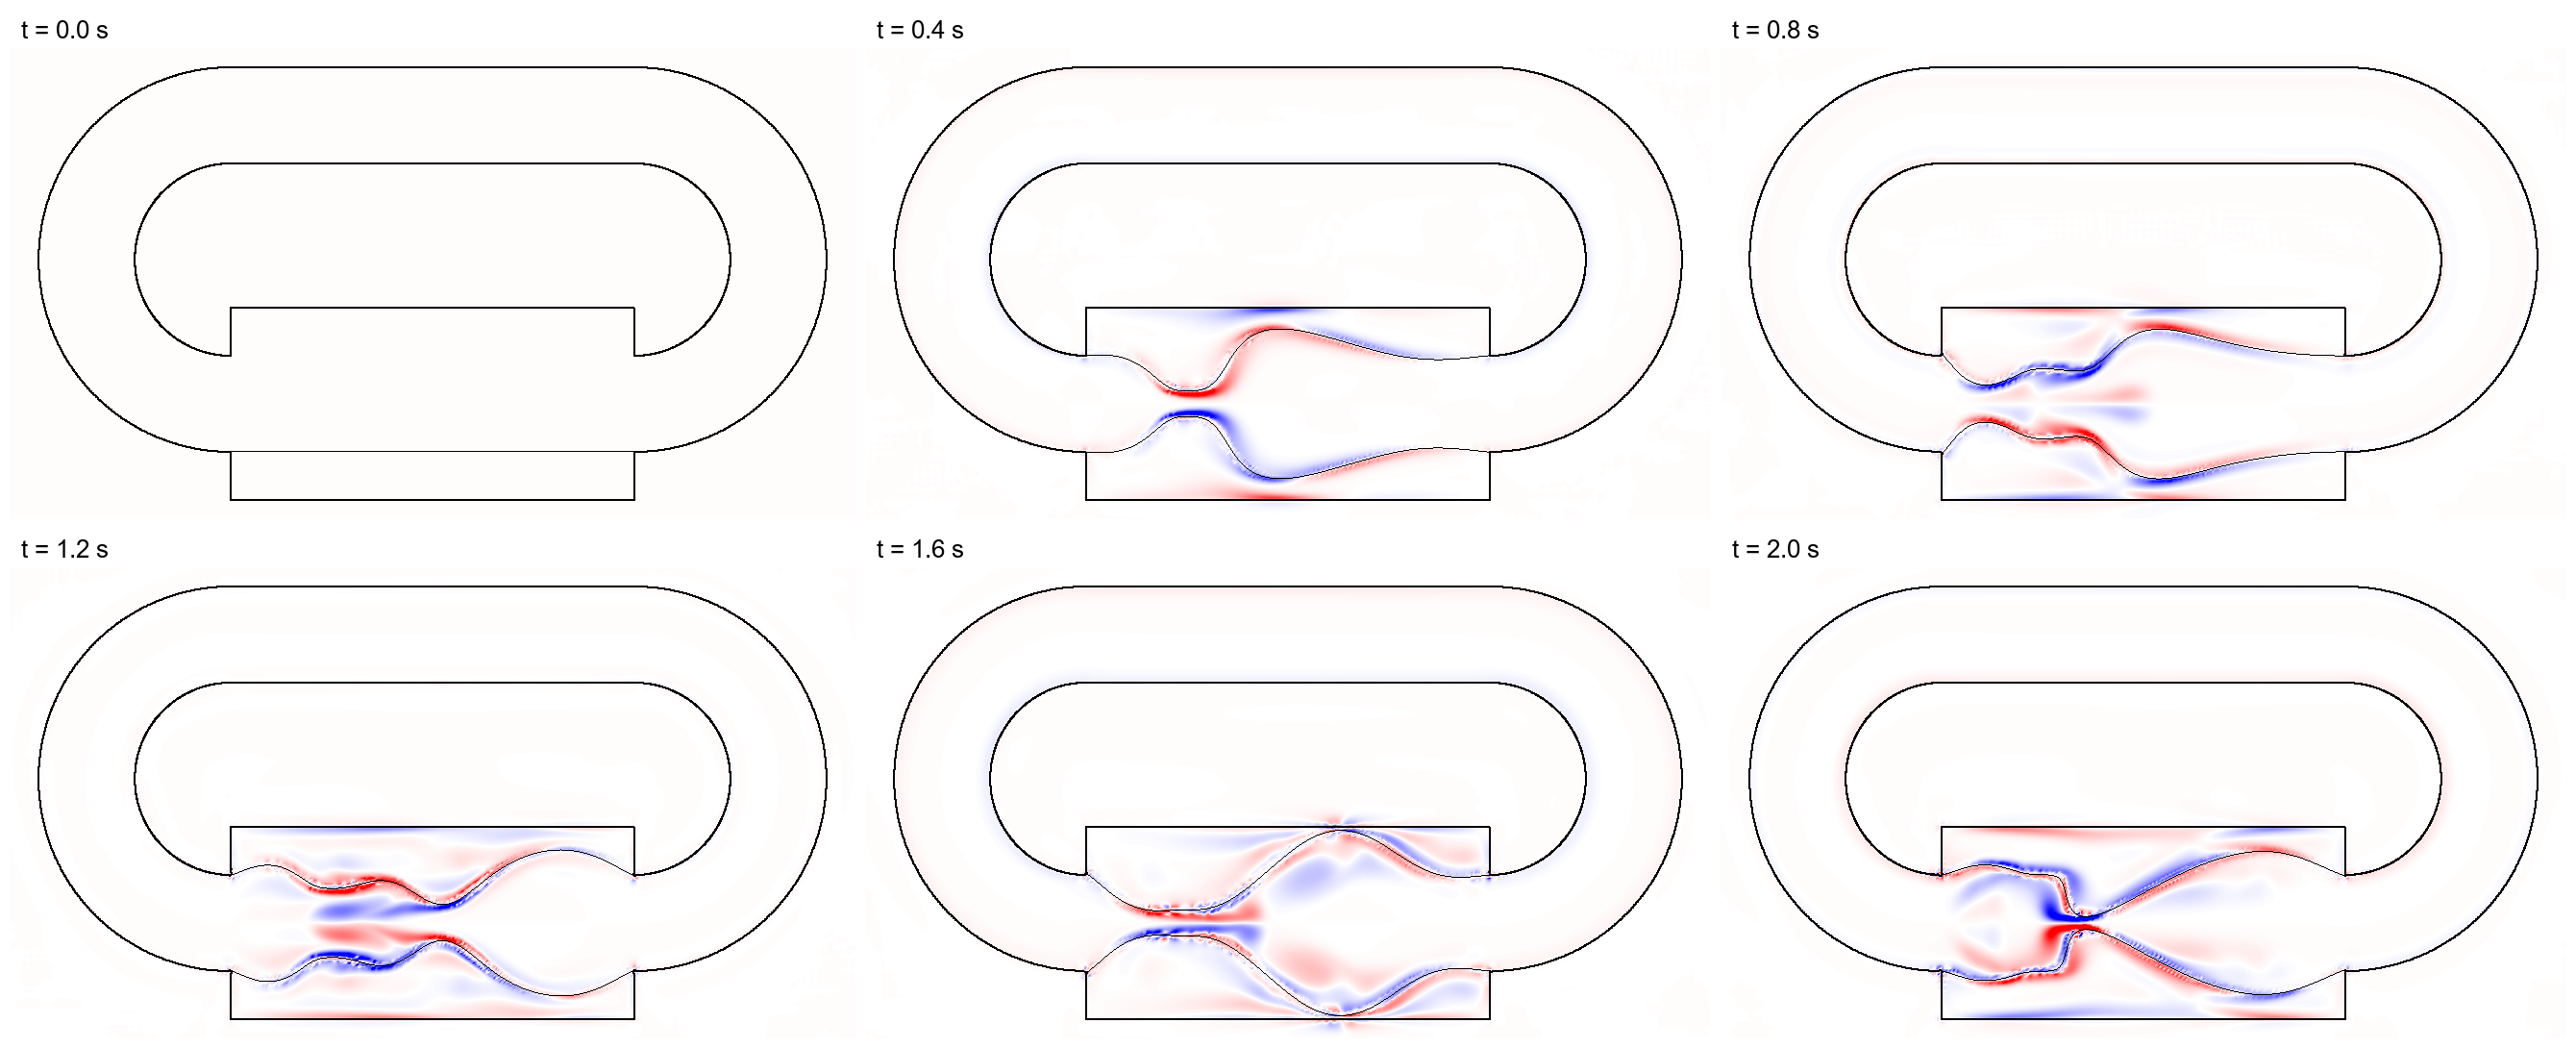
\includegraphics[width=\textwidth,height=0.6\textheight,keepaspectratio]{ch30-frames.png}

\footnotesize\raggedright
IB/11 (chapter 9b) in mode \code{TARGET\_VP}: a loop of tube 10 cm in diameter (the loop about 0.82 by 0.40 m), pumped by squeezing its elastic bottom section once a second; 2 s (two periods) at \code{DT} $= 5\times10^{-5}$ s with a dump every 800 steps (0.04 s): 51 dumps, so 51 frames. Shown: the vorticity \code{Omega} (colour table \code{difference}, fixed at $\pm103.1$ s$^{-1}$), the rigid racetrack (its vertices), the elastic tube (its spring mesh) and the rigid pericardium box. Above: dumps 0, 10, \dots, 50.
\sourcecredit{Frames by \code{wsl/final/ch30\_frames.sh} (VisIt 3.5.0, 1200 $\times$ 800); montage \code{tools/ch30\_figures.py}.}
\end{frame}

% 6
\begin{frame}{Three routes to the same frames}
\label{fr:routes}
\scriptsize
\begin{tabular}{@{}L{0.16\textwidth}L{0.24\textwidth}L{0.26\textwidth}L{0.24\textwidth}@{}}
\toprule
route & how & what you get & use it for \\
\midrule
1. the wizard & \gui{File $\to$ Save movie}, six pages for a simple movie (slides \ref{fr:wizard1}--\ref{fr:wizard2}) & a movie file, or the frames themselves if you choose an image format & one movie, now, from the GUI \\
2. \code{visit -movie} & a saved session (or a script) and one shell command (slides \ref{fr:vm}--\ref{fr:scriptfile}) & the same, without the GUI; \code{-source} swaps the data, but steps one time slider only (slide \ref{fr:sourcetrap}) & the same movie for several runs; a batch job \\
3. your own loop & \code{SaveWindow()} in a \code{for} loop, run by \code{visit -nowin -cli -s} (slides \ref{fr:loop}--\ref{fr:framescript}) & frames named as you like, and a table of their times & full control; the scripted analysis of chapters 27--29; the cluster \\
\bottomrule
\end{tabular}

\vspace{2mm}
\footnotesize
Routes 1 and 2 are the same program inside: the wizard writes a few lines of Python for the movie class of VisIt's \code{makemovie.py} (\code{movie.GenerateFrames()}, then \code{movie.EncodeFrames()}), which renders every frame and then calls ffmpeg through \code{visit\_utils/encoding.py}.
\begin{punchbox}
\small Whatever the route, ask for PNG frames and run ffmpeg yourself (slide \ref{fr:ffmpeg}): you keep the frames, you set the frame rate, and a new encoding takes a second instead of a new render.
\end{punchbox}
\sourcecredit{VisIt 3.5.0: \code{bin/makemovie.py}, \code{lib/site-packages/visit\_utils/encoding.py}, and the strings of \code{lib/libgui.so}.}
\end{frame}

% 7
\begin{frame}{Before the first frame}
\label{fr:before}
\footnotesize
\begin{enumerate}\setlength{\itemsep}{1pt}
  \item \gui{Options $\to$ Preferences}: untick \gui{Enable warning message popups}. Every old deck starts here: ``when we start saving movies, a pop-up will spring up every time-step''.
  \item Delete the Subset plot of \code{levels} that opening \code{dumps.visit} adds (slide \ref{fr:levels}).
  \item Fix the colour limits (slide \ref{fr:limits}).
  \item Fix the view: zoom once to the region that matters for the whole run (the structure moves). The view is saved with the session.
  \item One legend: keep the colour bar of the field, untick \gui{Legend} on the structure's plots. Waldrop: ``Most of the time, things like legends will need to be removed as to not clutter the plot.''
  \item A time stamp (slide \ref{fr:time}); no user name, no database path.
  \item The size in pixels: even numbers (H.264 needs them; slide \ref{fr:fftraps}), e.g.\ 1200 $\times$ 800 or 1920 $\times$ 1080, set in the wizard (\gui{Specify movie size}) or in the save options.
  \item Waldrop: ``Make sure that your Active Window is the window of the plot that you are trying to make the movie of.''
  \item Play it once with the time slider (2014: ``press the Play button and watch the simulation!''), then \gui{File $\to$ Save session}: the session is the movie's recipe, and route 2 replays it.
\end{enumerate}
\sourcecredit{The 2014--2024 tutorials and decks; Waldrop's guide.}
\end{frame}

% 8
\begin{frame}{Fix the colour limits}
\label{fr:limits}
\centering
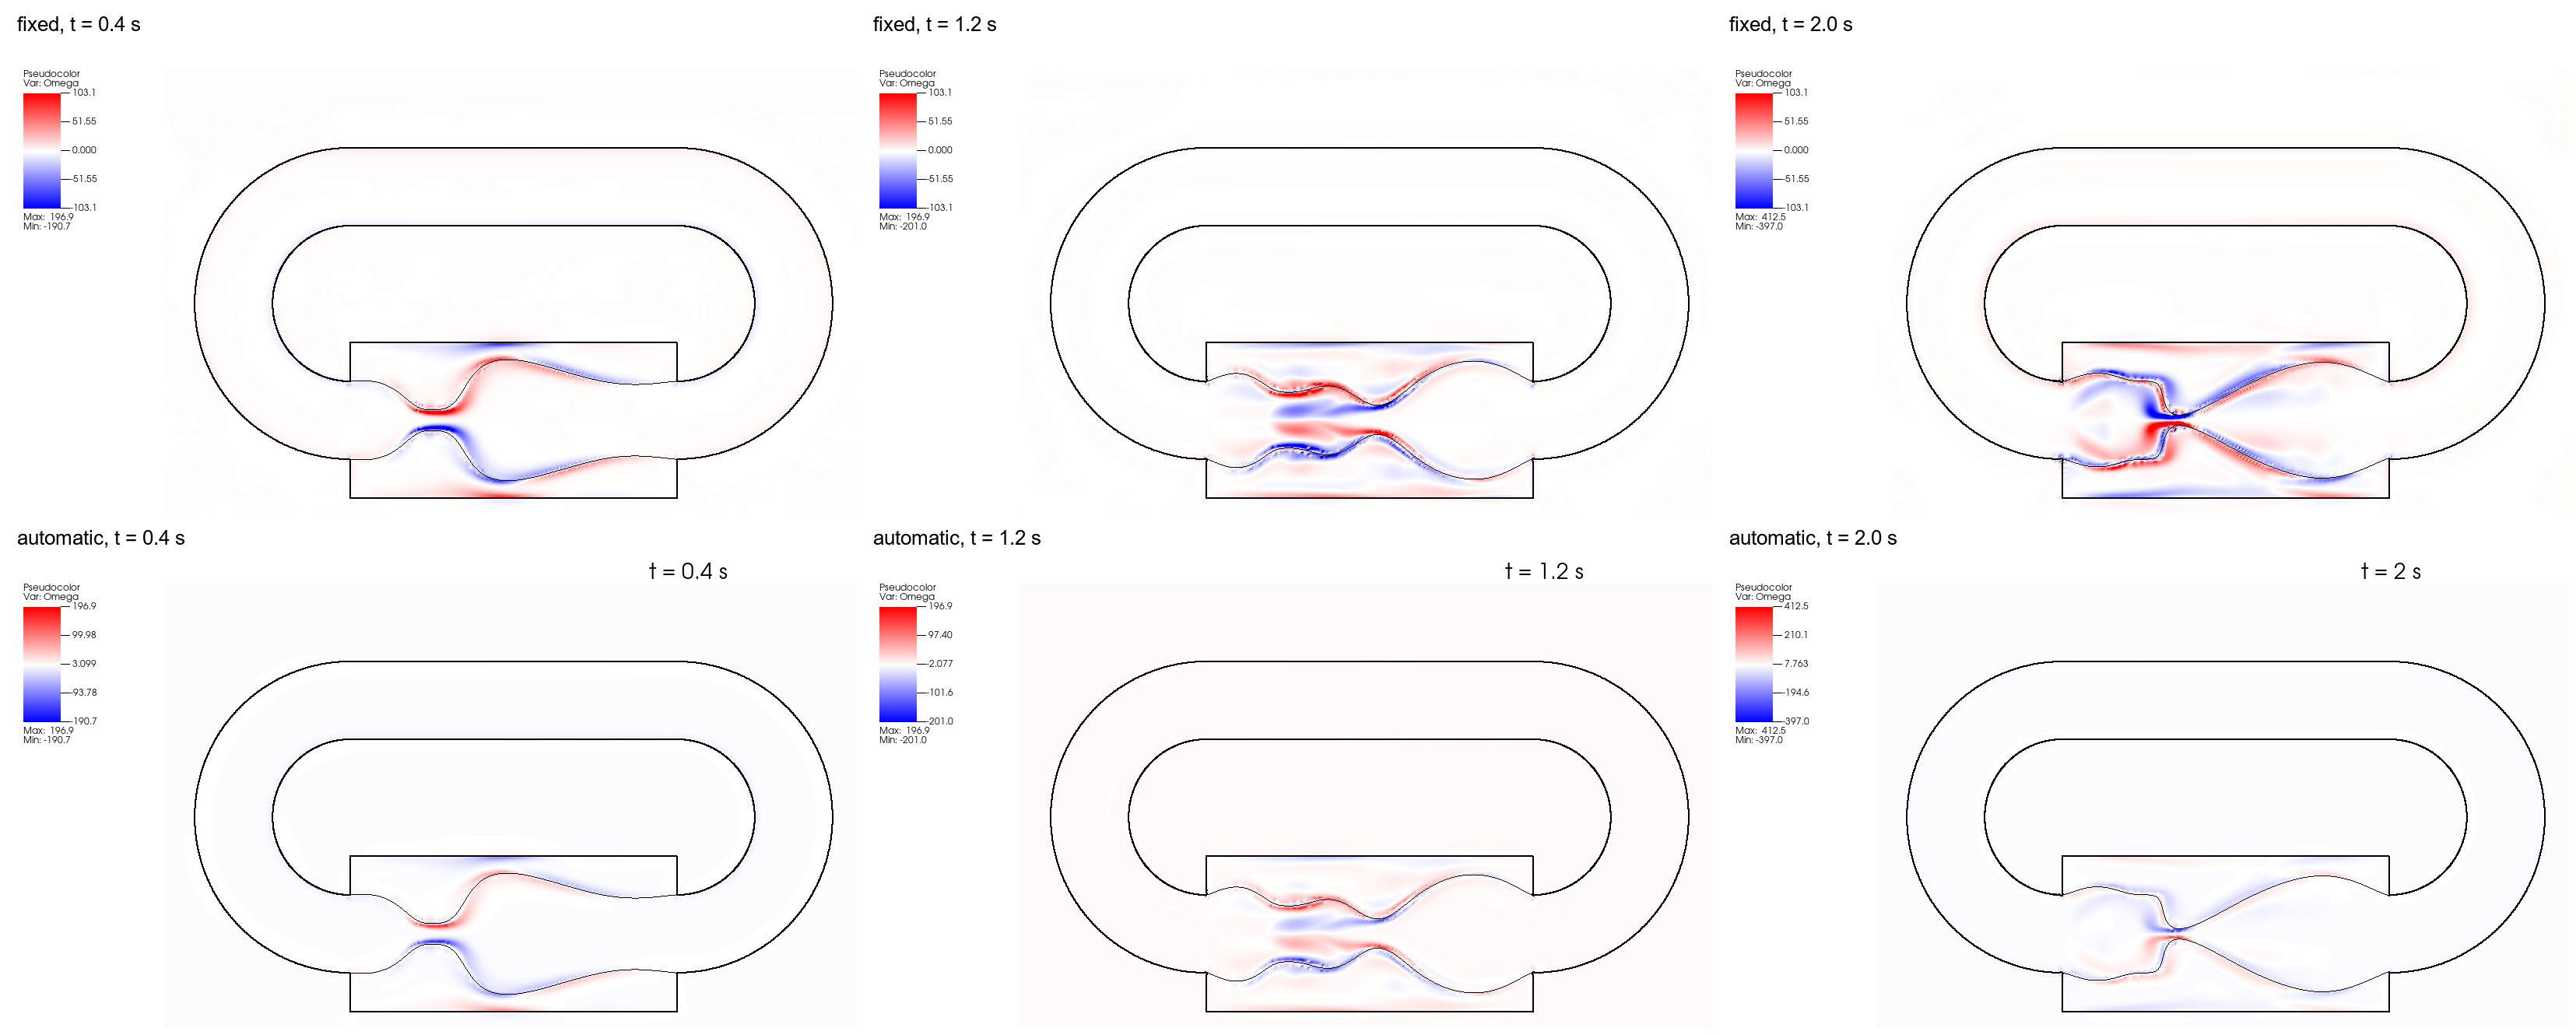
\includegraphics[width=\textwidth,height=0.52\textheight,keepaspectratio]{ch30-fixed-vs-auto.png}

\scriptsize\raggedright
\begin{itemize}\setlength{\itemsep}{0pt}
  \item \al{Automatic} limits follow each frame: $-190.7$ to $196.9$ at 0.4 s, $-201.0$ to $196.9$ at 1.2 s, $-397.0$ to $412.5$ at 2.0 s. In a movie the scale breathes: the same red means twice the vorticity at the end, and a strong vortex can look weaker than a faint one. An uneven range also moves zero off the white middle of \code{difference}, so the still fluid turns blue (middles $3.1$ and $7.8$) or pink ($-2.1$).
  \item \al{Fixed}: ``Try 25\% of original min/max'' (2020, slide 24): a quarter of the largest $|\Omega|$ at the last frame, $\pm103.1$ s$^{-1}$ (\gui{Limits}: tick \gui{Minimum} and \gui{Maximum}). The cores saturate: say so in the caption. The legend's \gui{Max} and \gui{Min} lines still report each frame's own extremes.
\end{itemize}
\sourcecredit{\code{wsl/final/ch30\_autolim.sh} (automatic limits, MinMax per frame) and \code{ch30\_frames.sh} (fixed).}
\end{frame}

% 9
\begin{frame}{The time stamp}
\label{fr:time}
\centering
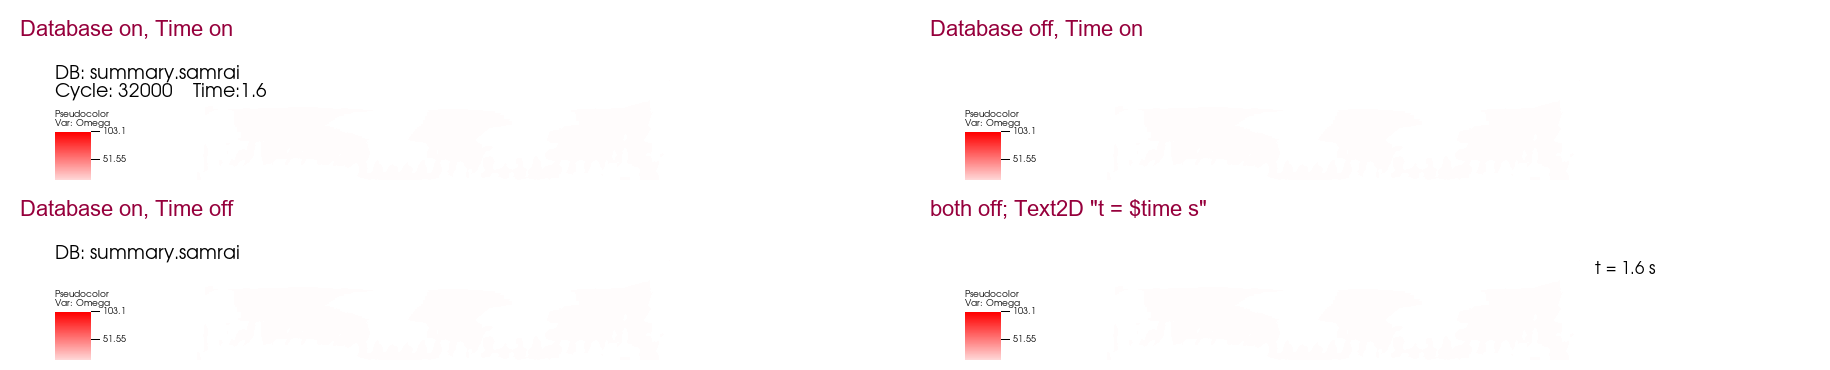
\includegraphics[width=\textwidth,height=0.3\textheight,keepaspectratio]{ch30-time-stamp.png}

\scriptsize\raggedright
\begin{itemize}\setlength{\itemsep}{1pt}
  \item In VisIt 3.5 the cycle and the time are printed only under the database's name (``DB: summary.samrai'', then ``Cycle: 32000\ \ Time:1.6''): untick \gui{Database} in \gui{Controls $\to$ Annotation $\to$ General} and they go too, whatever \gui{Time} says (top right).
  \item For the time alone: \gui{Controls $\to$ Annotation $\to$ Objects}, a \gui{Text 2D} object with the text \code{t = \$time s}. VisIt replaces \code{\$time} at every frame, in its shortest form: \code{t = 0.04 s}, \code{t = 1 s}, \code{t = 2 s} (the width changes, so put it where that does not matter). \code{\$cycle} gives the step (800, 20000, 40000) and \code{\$index} the dump (1, 25, 50, of \code{\$numstates} = 51).
  \item In a script: \code{t = CreateAnnotationObject("Text2D"); t.text = "t = \$time s"; t.position = (0.72, 0.92); t.height = 0.035}.
  \item The unit is yours to write: IBAMR's time is in the units of the input file (seconds for IB/11, which is in SI).
\end{itemize}
\sourcecredit{\code{wsl/final/ch30\_timeannot.sh} (dump 40, $t = 1.6$ s) and \code{ch30\_misc.sh} (dumps 1, 25, 50). Chapter 26 corrected to match.}
\end{frame}

% 10
\begin{frame}{The coloured lines: delete the Subset plot}
\label{fr:levels}
\centering
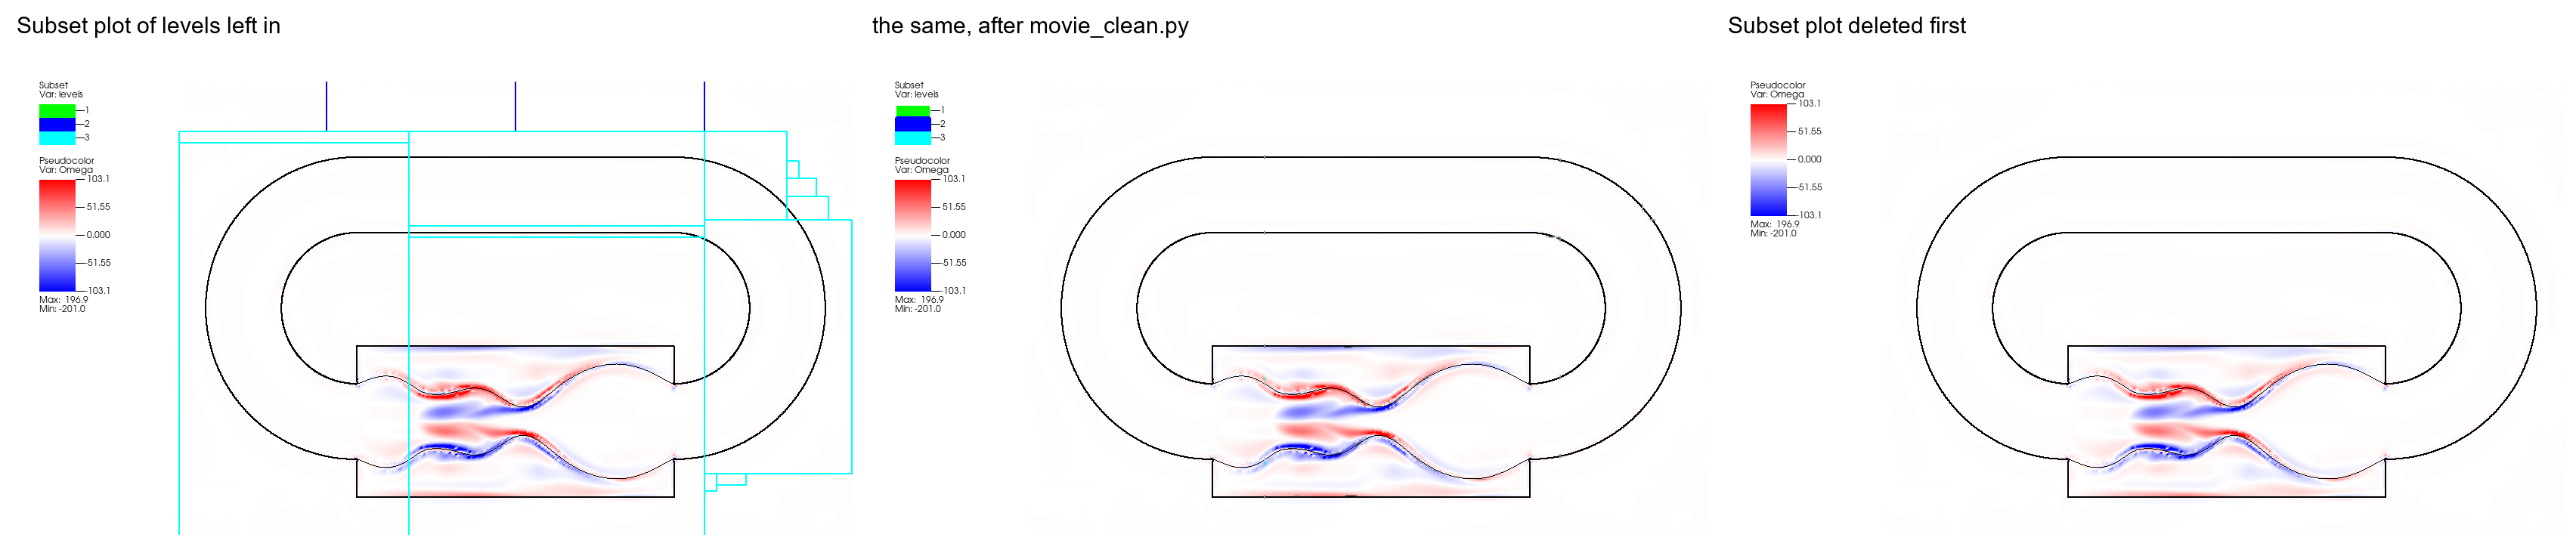
\includegraphics[width=\textwidth,height=0.36\textheight,keepaspectratio]{ch30-levels.png}

\footnotesize\raggedright
\begin{itemize}\setlength{\itemsep}{1pt}
  \item Opening \code{dumps.visit} adds a Subset plot of the variable \code{levels} by itself: the plot list right after \code{OpenDatabase} holds it (chapter 26). Its lines are the patch boundaries of the refinement levels, and they move at every regrid: the ``colored boxes'' of the 2014 tutorial, which it hid with \gui{Hide/Show}. Waldrop's guide deletes it: ``Most of the time, these just clutter your plot.
  \item For a movie, delete it: select it and \gui{Delete} in the GUI; \code{DeleteAllPlots()} right after \code{OpenDatabase} in a script (all of this chapter's scripts do).
  \item Frames already made: \code{examples/analysis/movie\_clean.py} (next slide) took the lines out of the left frame (middle), but not the Subset legend.
\end{itemize}
\sourcecredit{\code{wsl/final/ch30\_levels.sh}: dump 30 rendered with the Subset plot left in, then cleaned; right, the same dump from \code{ch30\_frames.sh}.}
\end{frame}

% 11
\begin{frame}{What the frame cleaner costs}
\label{fr:clean}
\centering
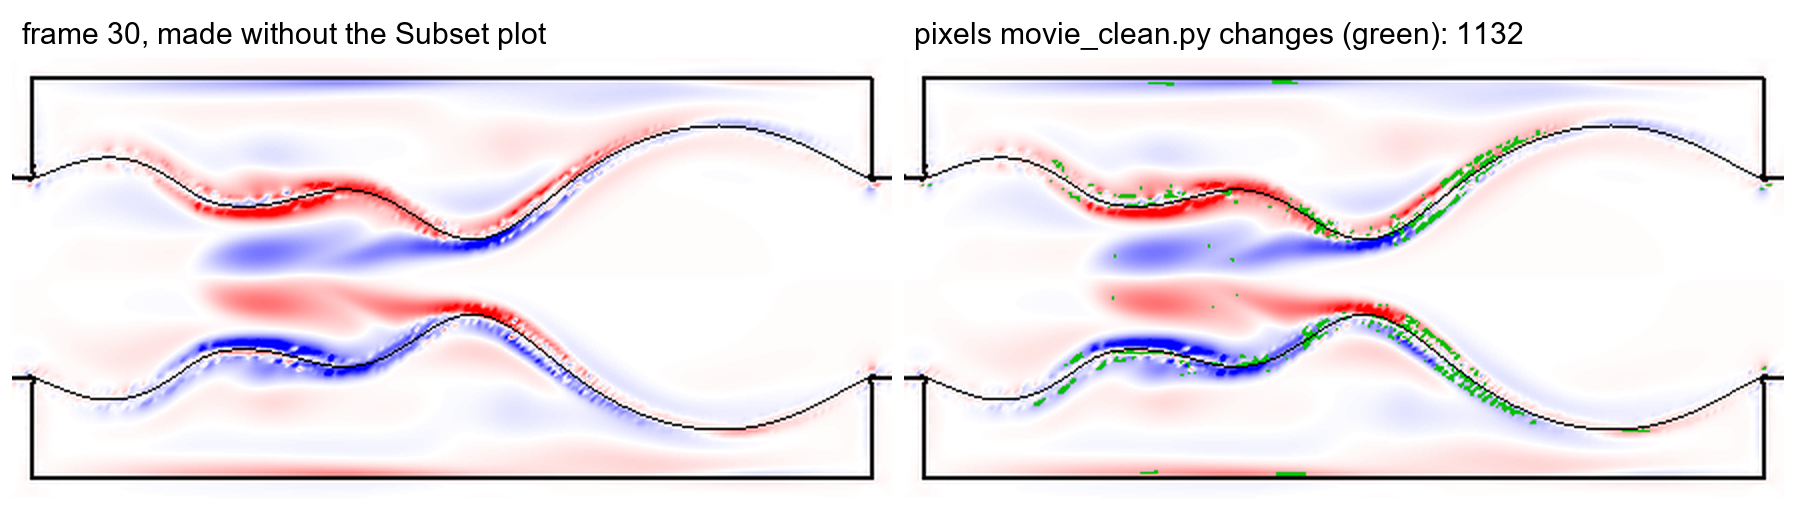
\includegraphics[width=0.92\textwidth,height=0.39\textheight,keepaspectratio]{ch30-clean-cost.png}

\footnotesize\raggedright
\begin{itemize}\setlength{\itemsep}{1pt}
  \item \code{python movie\_clean.py <frames folder> [glob, default f*.png] [K, default 1]} writes cleaned copies to \code{<folder>/clean/}. A line pixel is a saturated primary or secondary colour (red, green, blue, cyan, magenta, yellow) in a feature at most $2K$ pixels thick; it gets the mean colour of its neighbours. Green is always replaced (\code{difference} has none).
  \item The field's own thin saturated features look the same to it. On frames made without the Subset plot it still changed 691, 1132 and 1490 pixels (dumps 10, 30, 50): the saturated layers along the tube's walls, softened (above).
  \item So: a repair for old frames, not a step of the method. Delete the Subset plot and render again when you can.
\end{itemize}
\sourcecredit{\code{scratch/ch30/cleancheck} (the script run on three frames of \code{ch30\_frames.sh}); \code{tools/ch30\_figures2.py}.}
\end{frame}

% 12
\begin{frame}{Route 1: File $\to$ Save movie, pages 1 and 2}
\label{fr:wizard1}
\begin{columns}[T]
\column{0.44\textwidth}
\centering
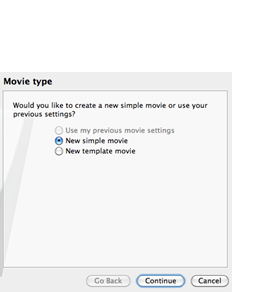
\includegraphics[height=0.37\textheight]{ch26-v2-movie-type.png}

\vspace{1mm}
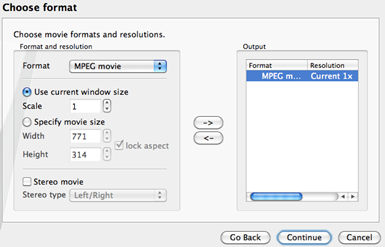
\includegraphics[width=\textwidth,height=0.37\textheight,keepaspectratio]{ch26-v2-movie-format.png}
\column{0.54\textwidth}
\scriptsize
\begin{itemize}\setlength{\itemsep}{1pt}
  \item \gui{File $\to$ Save movie} opens the \gui{Save movie wizard}.
  \item \gui{Movie type}: ``Would you like to create a new simple movie or use your previous settings?'' \gui{New simple movie}, \gui{Use my previous movie settings} (greyed out in the picture: there were no previous settings yet), or \gui{New template movie} (several viewports and sequences, set up from a movie template).
  \item \gui{Choose format}: a \gui{Format}, then the size: \gui{Use current window size} times a \gui{Scale}, or \gui{Specify movie size} with \gui{lock aspect}; \gui{Stereo movie} if you need it.
  \item Then the right arrow \gui{->}: the format goes into the \gui{Output} list. Waldrop: ``Be sure to click the -> button to add your movie to the queue.'' Several formats can be queued for one render, e.g.\ \gui{PNG images} and \gui{MP4 movie}.
  \item The formats VisIt 3.5 offers, and what they gave: slide \ref{fr:formats}.
\end{itemize}
\end{columns}
\sourcecredit{VisIt 2.5.2 windows from N. Battista's 2014 tutorial, reused in the 2020 deck (slides 21--22) and the 2024 practical (slides 25--26); the 3.5 page names and texts from \code{libgui.so}.}
\end{frame}

% 13
\begin{frame}{Route 1: pages 3 to 6}
\label{fr:wizard2}
\scriptsize
\begin{tabular}{@{}L{0.17\textwidth}L{0.79\textwidth}@{}}
\toprule
page & what it asks (VisIt 3.5) \\
\midrule
\gui{Choose length} & ``Choose movie start/end time and frames per second'': \gui{Frames per second}, \gui{First frame}, \gui{Last frame}, \gui{Frame stride} (2014: ``if you want to make a movie out of every other frame, every 5, etc''), \gui{Initial frame value} (the number of the first file) \\
\gui{Choose filename} & ``Choose the output directory and base filename for your movie(s)''; an image format adds the frame number: \code{racetrack0000.png}, \dots \\
\gui{E-mail notification} & ``Do you want to be notified by E-mail when your movie completes?'' (2014: ``Typically, I say no'') \\
\gui{Choose method} & ``Choose when and how you would like VisIt to create your movies'': \gui{Now, use currently allocated processors} (2014: ``What is easiest (and gives the least probability that Visit will get buggy and close)''); \gui{Now, use a new instance of VisIt} (``VisIt executed the following command line to begin making your movie''); \gui{Later, tell me the command to run} (``Execute the following command at the command prompt \dots'': a \code{visit -movie} command for route 2) \\
not in a simple movie & \gui{Save new template} (``Save this movie as a new template?''): only when you build a template movie; \gui{Settings check} (``Do these movie settings look okay?''): only after \gui{Use my previous movie settings}, where yes makes the movie and no goes back to \gui{Choose format} \\
\bottomrule
\end{tabular}

\vspace{1mm}
\footnotesize Then the frames are rendered one by one (Waldrop: on a Mac ``this will open a terminal window and begin making the plots one at a time'') and, for a movie format, encoded at the end. The frame rate you type here goes through the padding of slide \ref{fr:fps}.
\sourcecredit{Page names and quoted texts: VisIt 3.5.0's \code{libgui.so}; the order of the pages: \code{nextId()} in VisIt 3.5.0's \code{src/gui/QvisSaveMovieWizard.C}; the 2014 tutorial; Waldrop's guide.}
\end{frame}

% 14
\begin{frame}{The formats, and what they gave on 51 frames}
\label{fr:formats}
\scriptsize
VisIt 3.5's wizard lists \gui{PNG}, \gui{JPEG}, \gui{TIFF}, \gui{BMP}, \gui{PPM} and \gui{RGB images}, and \gui{MP4}, \gui{MPEG}, \gui{AVI}, \gui{DIVX}, \gui{GIF}, \gui{QuickTime}, \gui{SWF} and \gui{WMV movie}, all the movies but MPEG only when it finds \code{ffmpeg} on the PATH. The movies are made by ffmpeg: \code{encoding.py} offers mp4, mpg, wmv, gif, avi, mov, swf and divx only when \code{ffmpeg} is on the PATH, and MPEG falls back to VisIt's own \code{mpeg2encode} without it. VisIt renders JPEG frames for MP4, AVI, DIVX, GIF, SWF and WMV, and PNG frames for MPEG and QuickTime.

\vspace{1mm}
\begin{tabular}{@{}L{0.36\textwidth}L{0.25\textwidth}L{0.1\textwidth}L{0.08\textwidth}L{0.09\textwidth}@{}}
\toprule
how (1200 $\times$ 800) & codec & frames/s & length & size \\
\midrule
ffmpeg on the PNG frames, \code{-framerate 10} & H.264 High, yuv420p & 10 & 5.10 s & 0.56 MB \\
\code{visit -movie -format mp4} (\code{-fps 10}, the default) & H.264 High, yuv420p, from JPEG frames & 25, each frame 3 times & 6.12 s & 0.58 MB \\
\code{visit -movie -format mp4 -fps 30} & the same & 25 & 2.04 s & 0.38 MB \\
\code{visit -movie -format mpeg -fps 10} & MPEG-1, 2.6 Mbit/s (18 asked for) & 24 & 6.15 s & 2.0 MB \\
ffmpeg, a GIF 600 pixels wide & 256 colours & 10 & 5.10 s & 1.2 MB \\
ffmpeg without \code{-pix\_fmt yuv420p} & H.264 High 4:4:4 Predictive, yuv444p: QuickTime and most players refuse it & 10 & 5.10 s & 0.56 MB \\
\bottomrule
\end{tabular}

\vspace{1mm}
The PNG frames themselves: 4.0 MB for 51 (about 78 kB each). Rendering took 21 s; VisIt's MP4s 22--28 s with the encoding.
\sourcecredit{\code{wsl/final/ch30\_movies.sh}, \code{ch30\_movies4.sh}, \code{ch30\_mp4.sh}, \code{ch30\_examples.sh}; \code{ffprobe} for every number (the MPEG's bit rate: \code{scratch/ch30/verify\_agent/va\_run1.sh}).}
\end{frame}

% 15
\begin{frame}{The frame-rate trap}
\label{fr:fps}
\footnotesize
\code{makemovie.py}: ``We can only drive the movie at 30 fps. So if the user wants a movie at 10 fps, we have to pad frames.''
\begin{itemize}\setlength{\itemsep}{1pt}
  \item The padding: the smallest whole number $i$ with $30/i \le$ fps; each frame is copied $i$ times (3 for 10 frames/s, 1 for 30). A rate that is not 30 divided by a whole number prints ``Because of limitations in MPEG encoding, the movie will be encoded at \dots frames per second''.
  \item Then ffmpeg reads the copies at its default input rate for images, 25 per second (MP4), or writes MPEG-1 at 24 per second. Neither is 30.
  \item So \code{-fps 10} (and the wizard's \gui{Frames per second} 10) plays $25/3 = 8.3$ of your frames per second: 51 frames last 6.12 s, not 5.1. \code{-fps 30} plays 25 per second: 2.04 s.
\end{itemize}
\begin{punchbox}
\small If the rate matters (a period that should last a known time), make PNG frames and give ffmpeg the rate yourself: \code{-framerate 10} gives exactly 10 per second, 5.10 s.
\end{punchbox}
\sourcecredit{VisIt 3.5.0 \code{makemovie.py} (\code{EncodeMovie}, \code{EncodeMPEGMovie}) and \code{encoding.py} (\code{encode\_mp4}, \code{encode\_mpeg1}); measured with \code{wsl/final/ch30\_mp4.sh}, \code{ch30\_movies4.sh}.}
\end{frame}

% 16
\begin{frame}[fragile]{Route 2: \texttt{visit -movie} from a saved session}
\label{fr:vm}
\footnotesize
Set the plots up once (the GUI, or a script ending in \code{SaveSession("racetrack.session")}), save the session, then from a shell:
\begin{lstlisting}[style=shell,escapechar=!]
mkdir -p frames movies                               # the folders must exist (slide !\ref{fr:vmtraps}!)
visit -movie -format png -geometry 1200x800 \
      -sessionfile racetrack.session -output frames/f
# -> frames/f0000.png ... frames/f0050.png, one per dump
visit -movie -format png,mp4 -geometry 1200x800 -sessionfile racetrack.session -output movies/racetrack
\end{lstlisting}
\begin{itemize}\setlength{\itemsep}{1pt}
  \item \code{visit -help}: ``Run the CLI in a movie making mode. Must be combined with -sessionfile. Will produce a simple movie by drawing all the plots in the specified session for every timestep of the database.'' (\code{-scriptfile} works too: slide \ref{fr:scriptfile}.)
  \item In our runs (Linux, no display) adding \code{-nowin} changed nothing. On a cluster this is the command for a batch job (chapter 31); the wizard's \gui{Later, tell me the command to run} writes one for you.
  \item The session holds the plots, their attributes, the view, the annotations and the data files (\code{SOURCE00}, \code{SOURCE01}, \dots\ in the XML); \code{-source} replaces the data (slide \ref{fr:source}).
\end{itemize}
\sourcecredit{\code{wsl/final/ch30\_movies3.sh}, \code{ch30\_outdir.sh}; the help text of \code{visit} 3.5.0.}
\end{frame}

% 17
\begin{frame}{\texttt{visit -movie}: the options}
\label{fr:vmopts}
\scriptsize
\renewcommand{\arraystretch}{0.9}
\begin{tabular}{@{}L{0.27\textwidth}L{0.69\textwidth}@{}}
\toprule
option & what it does (from \code{makemovie.py}'s usage, VisIt 3.5) \\
\midrule
\code{-format f[,f2...]} & \code{png}, \code{jpeg}, \code{tiff}, \code{bmp}, \code{ppm}, \code{rgb} images; \code{mpeg}; with ffmpeg also \code{qt}, \code{mp4}, \code{wmv}, \code{gif}, \code{avi}, \code{swf}, \code{divx}; several at once with commas \\
\code{-geometry WxH[,W2xH2]} & the size; without it, the window size stored in the session (512 $\times$ 512 without a session) \\
\code{-sessionfile name} & the session to replay \\
\code{-source file} (repeat) & new data in place of the session's sources, in their order (only the active time slider is then stepped: slide \ref{fr:sourcetrap}); \code{-adjustview} resets the view to the new data's bounds, keeping the view normal and up vectors \\
\code{-scriptfile name}, \code{-templatefile name} & a Python script (slide \ref{fr:scriptfile}) or a movie template instead of a session \\
\code{-start}, \code{-end}, \code{-framestep} & which time states (the files are numbered from 0 unless \code{-frame} is given) \\
\code{-frame value} & the number of the first file \\
\code{-output name} & folder and base name of the frames or the movie \\
\code{-fps number} & the frame rate (default 10; slide \ref{fr:fps}) \\
\code{-stereo f} & \code{off}, \code{leftright}, \code{redblue}, \code{redgreen} \\
\code{-ignoresessionengines} & do not restart the compute engines stored in the session \\
\code{-email a,b} & progress reports by e-mail \\
\code{-noffmpeg} & MPEG through VisIt's own \code{mpeg2encode} \\
\code{-enginerestartinterval n} & restart the compute engine every $n$ images (memory, chapter 31) \\
\code{-np}, \code{-nn}, \code{-l}, \code{-la}, \code{-p} & a parallel engine: processors, nodes, the launcher (\code{mpirun}, \code{poe}, \code{psub}, \code{srun}), its arguments, the partition \\
\bottomrule
\end{tabular}
\sourcecredit{\code{makemovie.py} \code{PrintUsage} (VisIt 3.5.0): \code{wsl/final/ch30\_mmhelp.sh}, \code{ch30\_mmhelp2.sh}; \code{-fps} default from its source.}
\end{frame}

% 18
\begin{frame}{What \texttt{visit -movie} does not tell you (1/2)}
\label{fr:vmtraps}
\scriptsize
\begin{tabular}{@{}L{0.29\textwidth}L{0.35\textwidth}L{0.29\textwidth}@{}}
\toprule
what we did & what it printed & what it wrote \\
\midrule
\code{-output} into a folder that did not exist & ``Saved \dots/vm/frame0000.png'' for every frame, then ``VisIt completed generating frames'' & nothing, anywhere: create the folder first \\
\code{-sessionfile} naming a file that was not there & ``No image was saved. The combination of pixel data flags resulted in no image.'' \dots ``VisIt completed generating frames'' & nothing \\
\code{-scriptfile} with a script that only made the plots & ``VisIt completed generating frames'' & nothing (slide \ref{fr:scriptfile}) \\
\code{-start 10 -end 20 -framestep 5} & & \code{frame0000.png}--\code{frame0002.png} (dumps 10, 15, 20) \\
\bottomrule
\end{tabular}
\sourcecredit{\code{wsl/final/ch30\_movies.sh}, \code{ch30\_movies2.sh}, \code{ch30\_movies4.sh}, \code{ch30\_outdir.sh} (VisIt 3.5.0).}
\end{frame}

\begin{frame}{What \texttt{visit -movie} does not tell you (2/2)}
\label{fr:vmtraps2}
\scriptsize
\begin{tabular}{@{}L{0.29\textwidth}L{0.35\textwidth}L{0.29\textwidth}@{}}
\toprule
what we did & what it printed & what it wrote \\
\midrule
\code{-format png,mp4 -output movies/racetrack}, with \code{movies/} missing & a traceback ending ``FileNotFoundError: [Errno 2] No such file or directory: '\dots/movies''' & nothing: with a movie format VisIt lists the folder first, and stops \\
\code{-source} for another run with a structure & nothing unusual & frames whose structure stays at dump 0 (slide \ref{fr:sourcetrap}) \\
\code{-start 10 -end 20 -framestep 5 -frame 10 -output \dots/g} & & \code{g0010.png}--\code{g0012.png} \\
the runs from a session & ``ERROR: We could not parse the session file for engine launch parameters \dots\ Please report this.'' & the frames, correct: the message is harmless here \\
any run & & \code{<base>.log} in the working folder (\code{frame.log} for \code{-output \dots/frame}), and \code{visitlog.py}, as every CLI run \\
\bottomrule
\end{tabular}

\vspace{2mm}
\footnotesize Count the files after every run (\code{ls frames | wc -l}): ``completed'' does not mean ``written''.
\sourcecredit{\code{wsl/final/ch30\_outdir.sh}, \code{ch30\_source.sh}; \code{scratch/ch30/verify\_agent/va\_run2.sh} (D1) (VisIt 3.5.0).}
\end{frame}

% 19
\begin{frame}[fragile]{One session, another run: \texttt{-source}}
\label{fr:source}
\centering
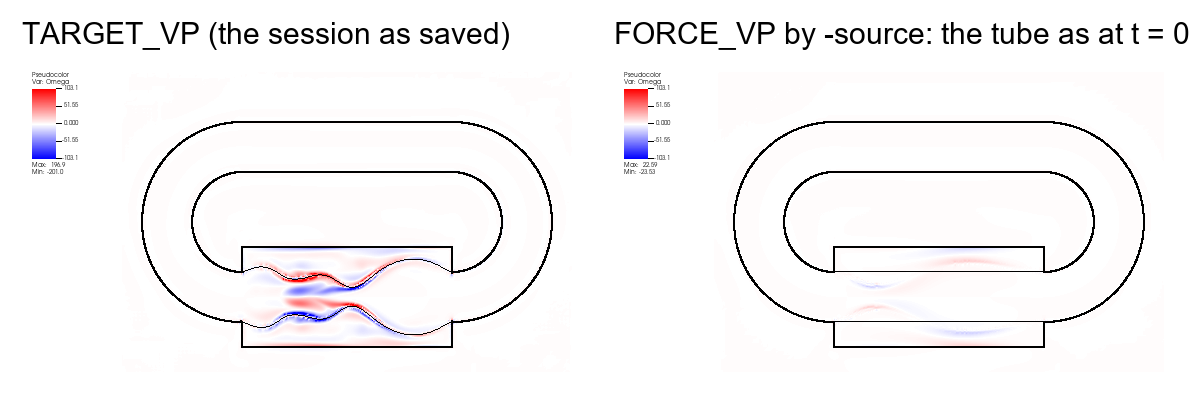
\includegraphics[width=0.8\textwidth,height=0.38\textheight,keepaspectratio]{ch30-side-by-side.png}
\raggedright
\begin{lstlisting}[style=shell]
visit -movie -format png -geometry 600x400 -sessionfile racetrack.session \
      -source FORCE_VP_F025/viz_IB2d/lag_data.visit -source FORCE_VP_F025/viz_IB2d/dumps.visit \
      -output force/frame                     # the session's SOURCE00 is lag_data.visit, SOURCE01 dumps.visit
ffmpeg -framerate 10 -i target/frame%04d.png -framerate 10 -i force/frame%04d.png \
       -filter_complex "[0:v][1:v]hstack=inputs=2" -c:v libx264 -pix_fmt yuv420p -crf 18 both.mp4
\end{lstlisting}
\scriptsize
51 frames of the force-driven pump in 14 s, with the session's plots, view and limits; then side by side, 1200 $\times$ 400, 5.1 s, 0.25 MB. Same limits on both sides is the point: at this dump $|\Omega|$ reaches 23.5 s$^{-1}$ in the force-driven pump and 201 in the target-driven one. \al{But the right-hand tube is straight, as at $t = 0$, in all 51 frames}: \code{-source} moved the fluid's time slider only (next slide).
\sourcecredit{\code{wsl/final/ch30\_source.sh}; IB/11's \code{FORCE\_VP} run with \code{Fmag\_vp} $= 0.25$ (chapter 9b).}
\end{frame}

% 19b
\begin{frame}[fragile]{\texttt{-source}: only one time slider moves}
\label{fr:sourcetrap}
\footnotesize
\begin{itemize}\setlength{\itemsep}{1pt}
  \item With \code{-source}, \code{makemovie.py} restores the session with the new files, re-opens each of them (``Restoring the session is messing up adding the new time sliders from the new databases to the new window''), then steps the \emph{active} time slider only (\code{IterateAndSaveFrames}: \code{SetTimeSliderState(i)}).
  \item The active slider is then the last file re-opened, the new \code{dumps.visit}: \code{SetTimeSliderState(25)} left \code{lag\_data.visit} and \code{Correlation01} at 0. In all 51 frames of the previous slide the force-driven tube's walls sit on the same pixel rows (239 and 289 of 400), as at $t = 0$; drawn at dump 30 they are squeezed.
  \item Without \code{-source} the replay is right: the \code{TARGET\_VP} frames are pixel for pixel those of the script (dumps 10, 15, 20 compared).
  \item For another run with a structure, step every slider: your own loop (slide \ref{fr:loop}), or \code{visit\_movie\_frames.py} with the session's limits, structures, view and size:
\end{itemize}
\begin{lstlisting}[style=shell]
visit -nowin -cli -s visit_movie_frames.py -- FORCE_VP_F025/viz_IB2d force lim=103.1 \
      meshes=heart_race_512_vertices,heart_tube_512_mesh,heart_peri_512_vertices \
      window=-0.45,0.45,-0.3,0.3 size=600x400 time=0 prefix=frame
\end{lstlisting}
\scriptsize 51 frames in 19.3 s, \code{force/frame0000.png} \dots\ \code{frame0050.png}; with the \code{TARGET\_VP} frames and the \code{hstack} command of the previous slide: 1200 $\times$ 400, 5.1 s, 0.26 MB, both tubes squeezed at dump 30.
\sourcecredit{VisIt 3.5.0 \code{makemovie.py} (\code{GenerateFrames}, \code{IterateAndSaveFrames}); \code{scratch/ch30/verify\_agent/va\_run6.sh}--\code{va\_run8.sh}; the walls' rows: \code{checks.py} there, on the frames of \code{ch30\_source.sh}.}
\end{frame}

\begin{frame}{The same dump, two ways}
\label{fr:sourcefix}
\centering
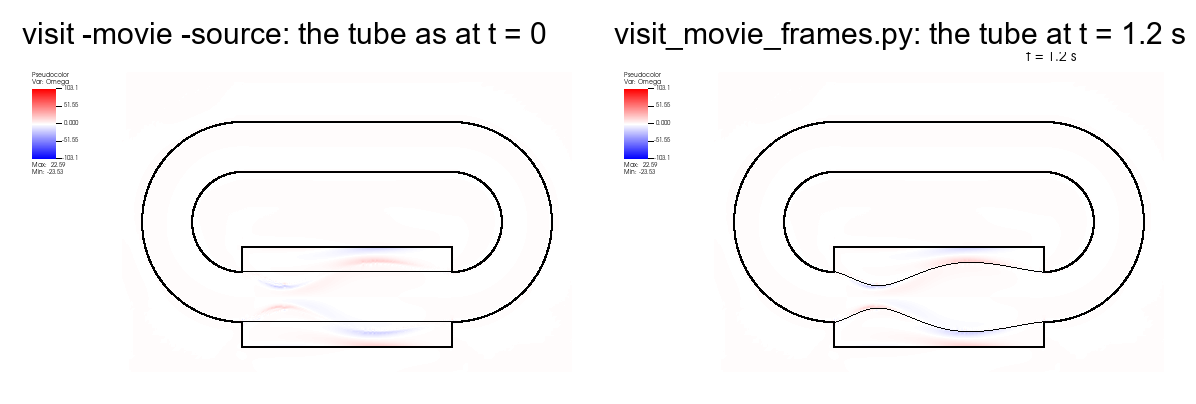
\includegraphics[width=\textwidth,height=0.5\textheight,keepaspectratio]{ch30-source-frozen.png}

\footnotesize\raggedright
\begin{itemize}\setlength{\itemsep}{1pt}
  \item \code{FORCE\_VP}, dump 30 ($t = 1.2$ s), the same limits and view. Left, from \code{visit -movie -source}: the fluid of dump 30 around the walls of dump 0. Right, from \code{visit\_movie\_frames.py}: the walls of dump 30, squeezed by the applied force.
  \item Nothing in the left frame looks wrong: the vorticity is right, the structure is plausible, and VisIt reported no problem. Only a frame from another route shows it. Check one frame of every new route against a frame you trust.
\end{itemize}
\sourcecredit{\code{scratch/ch30/verify\_agent} (\code{va\_run7.sh}, \code{va\_run8.sh}); \code{tools/ch30\_figures2.py}.}
\end{frame}

% 20
\begin{frame}[fragile]{\texttt{visit -movie -scriptfile}: your script steps through time}
\label{fr:scriptfile}
\footnotesize
With \code{-scriptfile} VisIt runs your script once, after replacing every \code{SaveWindow()} in it by its own numbered save (\code{CreateMangledSource} in \code{makemovie.py}). It does not step through time for you.
\begin{lstlisting}[style=pytiny,escapechar=!]
# ... OpenDatabase, DeleteAllPlots, AddPlot, attributes, DrawPlots, the view, the Text2D (as in the loop of slide !\ref{fr:loop}!)
for k in range(0, 51, 10):
    for ts in GetTimeSliders():
        SetActiveTimeSlider(ts); SetTimeSliderState(k)
    SaveWindow()
\end{lstlisting}
\begin{itemize}\setlength{\itemsep}{1pt}
  \item \code{visit -movie -nowin -format png -geometry 900x600 -scriptfile movie.py -output sf/frame}: 6 files, \code{frame0000.png}--\code{frame0005.png}, for dumps 0, 10, \dots, 50. The same script without the loop and \code{SaveWindow()}: no files.
  \item The rewrite keeps one character after \code{SaveWindow()} and drops the rest of the line, newline included. \code{SaveWindow(); n += 1} lost \code{n += 1} and glued the next line, \code{print(...)}, onto the end of the loop's last line: it printed six times, with \code{n} still 0.
  \item So write \code{SaveWindow()} exactly so, alone at the end of its line, and end the file with a newline: a script whose last line is \code{SaveWindow()} with no newline stopped with ``IndexError: string index out of range'' and wrote nothing.
\end{itemize}
\sourcecredit{\code{wsl/final/ch30\_scriptfile.sh}, \code{ch30\_scriptfile2.sh}; \code{makemovie.py} 3.5.0, \code{GenerateFrames} and \code{CreateMangledSource}.}
\end{frame}

% 21
\begin{frame}[fragile]{Route 3: your own loop}
\label{fr:loop}
\begin{columns}[T]
\column{0.55\textwidth}
\begin{lstlisting}[style=pytiny]
import os, sys; R = "viz_IB2d/"; os.makedirs("frames", exist_ok=True)
OpenDatabase(R + "lag_data.visit"); DeleteAllPlots()
OpenDatabase(R + "dumps.visit"); DeleteAllPlots()   # the levels plot
a = AnnotationAttributes()
a.userInfoFlag = 0; a.databaseInfoFlag = 0; a.axes2D.visible = 0
SetAnnotationAttributes(a)
t = CreateAnnotationObject("Text2D"); t.text = "t = $time s"
t.position = (0.72, 0.92); t.height = 0.035
AddPlot("Pseudocolor", "Omega"); p = PseudocolorAttributes()
p.colorTableName = "difference"; p.centering = p.Nodal
p.minFlag = 1; p.min = -103.1; p.maxFlag = 1; p.max = 103.1
SetPlotOptions(p); m = MeshAttributes(); m.legendFlag = 0
ActivateDatabase(R + "lag_data.visit")
AddPlot("Mesh", "heart_tube_512_mesh"); SetPlotOptions(m); DrawPlots()
v = GetView2D(); v.windowCoords = (-0.45, 0.45, -0.3, 0.3); SetView2D(v)
s = SaveWindowAttributes()
s.outputToCurrentDirectory = 0; s.outputDirectory = "frames"
s.family = 0; s.format = s.PNG
s.width, s.height = 1200, 800; s.resConstraint = s.NoConstraint
for k in range(TimeSliderGetNStates()):
    for ts in GetTimeSliders():       # fluid, structure, correlation
        SetActiveTimeSlider(ts); SetTimeSliderState(k)
    s.fileName = "f%04d" % k
    SetSaveWindowAttributes(s)
    SaveWindow()
sys.exit()
\end{lstlisting}
\column{0.43\textwidth}
\scriptsize
\begin{itemize}\setlength{\itemsep}{1pt}
  \item Run it with \code{visit -nowin -cli -s frames.py}. The \code{sys.exit()} at the end matters: without it the CLI waits at its prompt. \code{SaveWindow()} makes no folder: hence \code{os.makedirs}.
  \item \al{Every time slider}: with both files open, VisIt has one slider per database and a correlation of the two. Setting the active one alone left the others where they were (dumps.visit at 50, lag\_data.visit and the correlation at 0): a moving fluid around a frozen structure.
  \item \al{From dump 0}: the 2018 loop called \code{TimeSliderNextState()} before its first save (``to skip t=0''), so the initial state was never saved; it named the files with \code{family = 1} (VisIt numbers them: \code{visit0000.png}, \dots) and kept the window's proportions (\code{ScreenProportions}).
  \item Naming the files yourself ties frame $k$ to dump $k$; \code{NoConstraint} gives exactly the size asked for.
\end{itemize}
\end{columns}
\sourcecredit{The 2018 deck ``3B'', slide 7, rewritten for VisIt 3.5 (Python 3); time sliders: \code{wsl/final/ch30\_frames.sh}; the listing: \code{verify\_agent/va\_run1.sh}, \code{va\_run9.sh}.}
\end{frame}

% 22
\begin{frame}[fragile]{The loop as a script: \texttt{visit\_movie\_frames.py}}
\label{fr:framescript}
\begin{lstlisting}[style=pytiny]
visit -nowin -cli -s examples/analysis/visit_movie_frames.py -- <viz folder or dumps.visit> <out dir> [key=value ...]
    var=Omega  lim=auto  ct=difference  meshes=all  window=xmin,xmax,ymin,ymax  size=1200x800
    start=0 end=-1 every=1  first=0  time=1  legend=1  prefix=f  session=<file>
\end{lstlisting}
\scriptsize
\begin{itemize}\setlength{\itemsep}{1pt}
  \item \code{lim=auto}: a quarter of the largest $|$value$|$ at the last frame, the same for every frame (on IB/11: ``Omega at the last frame: min $-396.983$, max $412.509$; limits $-103.127$ .. $103.127$''); \code{lim=L} for $\pm L$; \code{lim=lo,hi}.
  \item \code{var=} also takes an expression: \code{"var=magnitude(U)" lim=0,0.5 ct=hot} for the speed (IBAMR 0.19 writes the vector \code{U} only).
  \item \code{meshes=all}: every \code{<name>\_mesh} of \code{lag\_data.visit}, and \code{<name>\_vertices} for structures without one (on IB/11 that adds the actuators and the markers); or a list: \code{meshes=heart\_race\_512\_vertices,heart\_tube\_512\_mesh,heart\_peri\_512\_vertices}; \code{meshes=none}.
  \item It deletes the Subset plot, writes \code{f0000.png}, \dots\ numbered without gaps whatever \code{every} is, and \code{frames.csv} (frame, dump, $t$); \code{first=} numbers a later chunk on (\code{start=25 end=50 first=25}: \code{f0025.png} \dots, \code{frames.csv} appended); \code{session=} also saves the set-up for \code{visit -movie}.
  \item On IB/11: 51 frames in 21.3 s; every fifth dump, 11 frames in 4.7 s.
\end{itemize}
\sourcecredit{\code{examples/analysis/visit\_movie\_frames.py}, tested by \code{wsl/final/ch30\_examples.sh} (VisIt 3.5.0).}
\end{frame}

% 23
\begin{frame}[fragile]{ffmpeg: one command, flag by flag}
\label{fr:ffmpeg}
\begin{lstlisting}[style=shell]
ffmpeg -framerate 10 -i frames/f%04d.png -c:v libx264 -pix_fmt yuv420p -crf 18 -movflags +faststart racetrack.mp4
\end{lstlisting}
\footnotesize
\begin{tabular}{@{}L{0.25\textwidth}L{0.71\textwidth}@{}}
\toprule
\code{-framerate 10} & before \code{-i}: how many frames go by per second (\code{-r} after \code{-i} changes the rate of the output by copying or dropping frames: slide \ref{fr:ffmore}) \\
\code{-i frames/f\%04d.png} & \code{f0000.png}, \code{f0001.png}, \dots, consecutive from 0 (or from \code{-start\_number N}) \\
\code{-c:v libx264} & H.264 video \\
\code{-pix\_fmt yuv420p} & colour at half resolution, the form players expect (slide \ref{fr:fftraps}) \\
\code{-crf 18} & the quality: 0 is lossless, 23 ffmpeg's default, 51 the worst; ``17 or 18'' is ``visually lossless or nearly so'' (FFmpeg's H.264 guide) \\
\code{-movflags +faststart} & the index at the front of the file, so a browser starts playing before the download ends \\
\bottomrule
\end{tabular}

\vspace{1mm}
On IB/11: 51 frames of 1200 $\times$ 800 $\to$ 5.10 s, 0.56 MB, in under a second. Getting ffmpeg: \code{sudo apt install ffmpeg} (Ubuntu, and WSL: 6.1.1 on Ubuntu 24.04), \code{brew install ffmpeg} (macOS), a Windows build linked from \url{https://ffmpeg.org/download.html} (add its \code{bin} folder to the PATH); on Puma, look with \code{module avail} (chapter 31).
\sourcecredit{\code{wsl/final/ch30\_movies.sh}; FFmpeg's H.264 encoding guide, \url{https://trac.ffmpeg.org/wiki/Encode/H.264}.}
\end{frame}

% 24
\begin{frame}{ffmpeg: the traps (1/2)}
\label{fr:fftraps}
\scriptsize
\begin{tabular}{@{}L{0.24\textwidth}L{0.36\textwidth}L{0.33\textwidth}@{}}
\toprule
what we did & what happened & what to do \\
\midrule
frames of 1199 $\times$ 799 & ``width not divisible by 2 (1199x799)'', ``Error while opening encoder'', and an empty (0-byte) file & \code{-vf "pad=ceil(iw/2)*2:ceil(ih/2)*2"} (adds a pixel; VisIt's own MP4 encoder does this) or \code{scale=trunc(iw/2)*2:trunc(ih/2)*2} (1198 $\times$ 798) \\
no \code{-pix\_fmt} on PNG frames & H.264 ``High 4:4:4 Predictive'', yuv444p: full colour resolution, which ``QuickTime and most other players'' do not play (FFmpeg's guide) & always \code{-pix\_fmt yuv420p} \\
frames 0, 1, 3 (2 missing) & \code{-i f\%04d.png} stopped at the gap: 2 frames & renumber, or \code{-pattern\_type glob -i "f*.png"} (3 frames; needs an ffmpeg built with globbing, which the usual Windows builds are not), or \code{make\_movie.py} \\
\bottomrule
\end{tabular}
\sourcecredit{ffmpeg 6.1.1 on the IB/11 frames: \code{wsl/final/ch30\_movies.sh}; \url{https://trac.ffmpeg.org/wiki/Encode/H.264}.}
\end{frame}

\begin{frame}{ffmpeg: the traps (2/2)}
\label{fr:fftraps2}
\scriptsize
\begin{tabular}{@{}L{0.24\textwidth}L{0.36\textwidth}L{0.33\textwidth}@{}}
\toprule
what we did & what happened & what to do \\
\midrule
frames that start at 10 & ``Could find no file with path 'f\%04d.png' and index in the range 0-4'', and no file & \code{-start\_number 10} (41 frames from \code{f0010.png}) \\
\code{-framerate 10} after \code{-i} & no error; the images went by at ffmpeg's default for images, 25 per second: 51 frames in 2.04 s & \code{-framerate} before \code{-i} \\
UArizona's VisIt page: \code{ffmpeg -f image2 -i movie\%04d.png -r 10 output.mp4} & the images read at 25 per second, then thinned to 10: 22 of the 51 frames kept, 2.2 s; and yuv444p & \code{-framerate 10} before \code{-i}, and \code{-pix\_fmt yuv420p}: 51 frames, 5.1 s \\
\bottomrule
\end{tabular}
\sourcecredit{ffmpeg 6.1.1 on the IB/11 frames: \code{wsl/final/ch30\_movies.sh}, \code{ch30\_misc.sh}, \code{ch30\_uahpc\_ffmpeg.sh}; \url{https://trac.ffmpeg.org/wiki/Encode/H.264}; UArizona HPC documentation, VisIt page (read 17 October 2026).}
\end{frame}

% 25
\begin{frame}[fragile]{More with ffmpeg (1/2)}
\label{fr:ffmore}
\begin{lstlisting}[style=pytiny,escapechar=!]
# a GIF with its own 256-colour palette, 600 pixels wide          -> 1.2 MB (the full-size MP4: 0.56 MB)
ffmpeg -framerate 10 -i f%04d.png -vf "scale=600:-1:flags=lanczos,split[a][b];[a]palettegen[p];[b][p]paletteuse" race.gif
# two runs side by side (slide !\ref{fr:source}!); vstack=inputs=2 puts them one above the other
ffmpeg -framerate 10 -i a/f%04d.png -framerate 10 -i b/f%04d.png -filter_complex "[0:v][1:v]hstack=inputs=2" \
       -c:v libx264 -pix_fmt yuv420p both.mp4
# twice as slow: every frame shown twice as long                 -> 10.1 s instead of 5.1
ffmpeg -framerate 10 -i f%04d.png -vf "setpts=2*PTS" -c:v libx264 -pix_fmt yuv420p slow.mp4
# the same 51 frames at 30 frames/s: each repeated three times    -> 153 frames, still 5.1 s, no smoother
ffmpeg -framerate 10 -i f%04d.png -r 30 -c:v libx264 -pix_fmt yuv420p r30.mp4
\end{lstlisting}
\scriptsize Smoothness comes from more frames (more dumps), never from \code{-r} or \code{setpts}: slide \ref{fr:rate}.
\sourcecredit{All run on the IB/11 frames with ffmpeg 6.1.1: \code{wsl/final/ch30\_movies.sh}, \code{ch30\_source.sh}, \code{ch30\_misc.sh}.}
\end{frame}

\begin{frame}[fragile]{More with ffmpeg (2/2)}
\label{fr:ffmore2}
\begin{lstlisting}[style=pytiny]
# a region only: width:height:x:y in pixels (the elastic section)  -> 440 x 220
ffmpeg -framerate 10 -i f%04d.png -vf "crop=440:220:470:420" -c:v libx264 -pix_fmt yuv420p tube.mp4
# one frame back out of a movie (frame 30, counted from 0)
ffmpeg -i tube.mp4 -vf "select=eq(n\,30)" -vframes 1 tube_030.png
# a title card shown for 2 s, then the movie (title.png the same size as the frames)  -> 71 frames, 7.1 s
ffmpeg -loop 1 -framerate 10 -t 2 -i title.png -framerate 10 -i f%04d.png \
       -filter_complex "[0:v][1:v]concat=n=2:v=1:a=0,format=yuv420p" -c:v libx264 -crf 18 titled.mp4
\end{lstlisting}
\scriptsize
\begin{itemize}\setlength{\itemsep}{1pt}
  \item The title card is any picture of the frames' size (a slide exported as PNG, or made in Python): what is shown, the run, the units, the slowdown and the colour limits, for the viewer who sees the movie without your talk. \code{-loop 1 -t 2} turns the still into 2 s of video at the movie's rate; \code{concat} joins the two.
  \item Chapter 4b promised the title frame here: it is the ``what am I looking at'' that a movie on a web page or in a supplement does not otherwise have.
\end{itemize}
\sourcecredit{ffmpeg 6.1.1 on the IB/11 frames: \code{wsl/final/ch30\_misc.sh}, \code{ch30\_title.sh}; the crop: \code{scratch/ch30/verify\_agent/va\_run3.sh}.}
\end{frame}

% 26
\begin{frame}[fragile]{\texttt{make\_movie.py}: frames to a movie on any system}
\label{fr:makemovie}
\begin{lstlisting}[style=shell]
python make_movie.py frames                                  # frames/*.png -> frames/movie.mp4 at 10 frames/s
python make_movie.py frames --glob "f*.png" --fps 25 --crf 18 --out racetrack.mp4
python make_movie.py frames --gif --width 600 --out racetrack.gif
\end{lstlisting}
\footnotesize
\begin{itemize}\setlength{\itemsep}{1pt}
  \item It copies the frames, in name order, to a temporary folder as \code{00000.png}, \code{00001.png}, \dots\ (so gaps and odd first numbers do not matter, and no glob is needed), pads the size to even numbers, sets \code{-pix\_fmt yuv420p}, prints the ffmpeg command it runs and the movie's length and size.
  \item Tested (ffmpeg 6.1.1) on the frames of \code{visit\_movie\_frames.py}: 51 frames $\to$ 5.10 s, 571 kB, H.264 High, yuv420p, 10 frames/s; every other frame of the first 50 (25 files) $\to$ 25 frames; frames of 601 $\times$ 401 $\to$ a movie of 602 $\times$ 402; \code{--gif --width 600} $\to$ 1208 kB.
  \item It needs Python 3 and ffmpeg on the PATH, nothing else; it says where to get ffmpeg if it is missing.
\end{itemize}
\sourcecredit{\code{examples/analysis/make\_movie.py}, tested by \code{wsl/final/ch30\_examples.sh} (Ubuntu 24.04 in WSL).}
\end{frame}

% 27
\begin{frame}{Choosing the frame rate and the dump interval}
\label{fr:rate}
\footnotesize
\begin{itemize}\setlength{\itemsep}{1pt}
  \item One frame per dump. IB/11's 51 dumps at 10 frames/s last 5.1 s: each 0.04 s of the run is shown for 0.1 s, so the run is slowed 2.5 times, one pumping period in 2.5 s. At 25 frames/s (real time) the whole run is over in 2.04 s.
  \item Rates of 10 to 30 frames/s are usual; at the low end the motion is jerky. Slowing a few frames down (\code{setpts}, \code{-r}) does not add motion between them.
  \item Plan backwards from the movie: length $\times$ rate = frames; the run's time / frames = the dump interval. A 10 s movie of IB/11 at 25 frames/s needs 250 frames over 2 s: a dump every 0.008 s, \code{VIZ\_INTERVAL = 160} steps of $5\times10^{-5}$ s in its input (now \code{int(END\_TIME/(50*DT))} $= 800$).
  \item The disk: IB/11's dumps are about 2.5 MB each, 2.6 MB with the structure's files (133 MB for 51); 250 would be about 650 MB. A 3D run's dumps are far bigger: dump often only over the interval the movie shows (restart from a restart file with a smaller interval in the input, chapter 3; IB/11 writes none, \code{restart\_dump\_interval = 0}, so set it before the run; after a restart \code{dumps.visit} lists only the later dumps, chapter 33), or make the frames as the run goes and keep fewer dumps.
  \item Write the slowdown in the caption: ``2 s of simulated time shown in 5.1 s''.
\end{itemize}
\sourcecredit{IB/11's input (\code{DT}, \code{END\_TIME}, \code{VIZ\_INTERVAL}) and \code{du -sb} of its \code{viz\_IB2d} folder (\code{scratch/ch30/verify\_agent/va\_run1.sh}).}
\end{frame}

% 28
\begin{frame}{Movies in talks, papers and on the web}
\label{fr:talks}
\footnotesize
\begin{itemize}\setlength{\itemsep}{1pt}
  \item \al{Slides}: H.264 in an MP4 with \code{yuv420p} is the format PowerPoint, Keynote and web browsers all play. Test it on the computer you will present from, and put a still of the key frame on a backup slide.
  \item \al{Beamer and PDF}: most PDF viewers do not play embedded video; link the file and play it in a player, or show the still with the link.
  \item \al{Papers}: supplementary movies as MP4; read the journal's limits on size and format first. Keep the frames: a figure panel is a frame you already have.
  \item \al{The web and social media}: MP4 with \code{+faststart}; a GIF only for a short loop (ours is twice the size of the MP4 at half the width).
  \item \al{The caption}: the variable and its colour limits (``saturated at $\pm103$ s$^{-1}$''), the time stamp's units, the slowdown, the run (the data sheet of chapter 29).
  \item \al{The record}: keep the session or the script, the frames (or the command that remakes them) and the encoding command beside the run. Waldrop's rule holds for movies too: someone else should be able to remake it without asking you.
\end{itemize}
\end{frame}

% 29
\begin{frame}{Movies on the cluster}
\label{fr:cluster}
\footnotesize
\begin{itemize}\setlength{\itemsep}{1pt}
  \item Every route but the wizard runs without a display: \code{visit -nowin -cli -s visit\_movie\_frames.py -- \dots} or \code{visit -movie \dots} inside a batch job, next to the data (the dumps of a 3D run are too big to copy home just for a movie).
  \item \code{visit -movie} can launch a parallel compute engine itself: \code{-np}, \code{-nn}, \code{-l srun}, \code{-la}, \code{-p} (slide \ref{fr:vmopts}).
  \item Long movies: \code{-enginerestartinterval n} restarts the compute engine every $n$ images (for a render that slows down or runs out of memory), and a script can do its frames in chunks, each with its own \code{start=}, \code{end=} and \code{first=}.
  \item Encode on the cluster if it has ffmpeg, or copy the frames home (4.0 MB for our 51) and encode there.
  \item Puma's VisIt module, client--server use and a Slurm script for frames: chapter 31.
\end{itemize}
\sourcecredit{\code{makemovie.py}'s usage (VisIt 3.5.0); the 2018 deck ``3B'', slide 8 (a VisIt script run on Killdevil).}
\end{frame}

% 30
\begin{frame}{When the movie goes wrong}
\label{fr:trouble}
\scriptsize
\begin{tabular}{@{}L{0.4\textwidth}L{0.55\textwidth}@{}}
\toprule
what you see & what to do \\
\midrule
a pop-up at every frame & untick \gui{Enable warning message popups} (slide \ref{fr:before}) \\
coloured straight lines that jump around & delete the Subset plot of \code{levels} (slide \ref{fr:levels}) \\
the colours flicker, or the still fluid changes colour & fixed limits (slide \ref{fr:limits}) \\
no time on the frames & a \gui{Text 2D} with \code{\$time} (slide \ref{fr:time}) \\
``completed'' or ``Saved'', but no files & create the output folder: VisIt does not, in \code{visit -movie} or in your own loop (ours printed ``Saved'' 51 times and wrote nothing); check the session's path; a \code{-scriptfile} must call \code{SaveWindow()} (slide \ref{fr:vmtraps}) \\
the fluid moves, the structure does not & set every time slider (slide \ref{fr:loop}); after \code{visit -movie -source}, make the frames with your own loop (slide \ref{fr:sourcetrap}) \\
the movie plays slower (and lasts longer) than asked & VisIt's padding (slide \ref{fr:fps}): give the rate to ffmpeg \\
``width not divisible by 2'' & pad to even sizes (slide \ref{fr:fftraps}) \\
the MP4 will not play in QuickTime or another player & \code{-pix\_fmt yuv420p} \\
ffmpeg makes a movie of only the first few frames & a gap in the numbering: renumber or \code{make\_movie.py} \\
a jerky movie & more dumps, not a lower rate (slide \ref{fr:rate}) \\
the legend's numbers change from frame to frame & they are the frame's \gui{Max} and \gui{Min}: the limits are on the bar's ends \\
\bottomrule
\end{tabular}
\sourcecredit{The 2014--2024 decks and what happened while this chapter was made (VisIt 3.5.0, ffmpeg 6.1.1).}
\end{frame}

% 31
\begin{frame}{Exercises}
\label{fr:exercises}
\footnotesize
\begin{enumerate}\setlength{\itemsep}{1pt}
  \item Make the IB/11 vorticity movie three ways (the wizard with PNG images, \code{visit -movie} from your saved session, \code{visit\_movie\_frames.py}), encode each with ffmpeg at 10 frames/s, and compare the frames and the files.
  \item Ask the wizard (or \code{visit -movie}) for an MP4 at 10 frames/s and measure its length with \code{ffprobe}. Explain the number.
  \item Make a movie with automatic limits and one with fixed limits; watch both. Which vortex looks strongest in each, at 1.2 s and at 2.0 s?
  \item Replay your session on IB/11's \code{FORCE\_VP} run with \code{-source} and put the two movies side by side. What do the same limits show that separate limits would hide? Does the tube move? Make the \code{FORCE\_VP} frames again with \code{visit\_movie\_frames.py} (same limits and view) and compare.
  \item Make a movie of the speed, \code{magnitude(U)}, with the \code{hot} colour table, fixed limits 0 to 0.5 m/s and the markers drawn as points.
  \item Plan a 10 s movie of one pumping period at 25 frames/s: the dump interval, the number of dumps, the disk. Rerun IB/11 for one period with that interval and make it.
  \item Crop the movie to the elastic section and make a GIF of it under 1 MB.
  \item Write the caption and the record (session, commands, data sheet) for one of your movies, so that someone else could remake it.
\end{enumerate}
\end{frame}

% 32
\begin{frame}{Summary}
\label{fr:summary}
\footnotesize
\begin{itemize}\setlength{\itemsep}{1pt}
  \item A movie is frames plus an encoder. Make PNG frames (the wizard with an image format, \code{visit -movie -format png}, or your own loop), keep them, and encode with ffmpeg: \code{-framerate}, \code{libx264}, \code{yuv420p}, \code{-crf 18}, \code{+faststart}.
  \item Before the first frame: no pop-ups, no Subset plot, fixed limits, a fixed view, one legend, a \code{\$time} stamp, an even size.
  \item VisIt's own movie formats pad frames for 30 frames/s and are read back at 25 per second (MPEG is written at 24): the rate you get is not the rate you typed. Its MPEG is MPEG-1 and 3.6 times the size of an H.264 MP4.
  \item \code{visit -movie} replays a session (\code{-start}, \code{-end}, \code{-framestep}, \code{-frame}; \code{-source} for another run, but it steps one time slider only: our structure stayed at dump 0); it says ``completed'' when it wrote nothing, so count the files. With \code{-scriptfile} your script loops and calls \code{SaveWindow()} on its own line.
  \item Choose the movie first (its length and rate), then the dump interval, and write the slowdown and the limits in the caption.
\end{itemize}
\begin{punchbox}
\small The old advice holds: ``Save as mpeg is not the best option.'' Save the frames, and let ffmpeg make the movie.
\end{punchbox}
\end{frame}

% 33
\begin{frame}{References and credits}
\label{fr:refs}
\scriptsize
\begin{itemize}
  \item N. Battista, ``Part III: Let's make groovy movies! -- Visualizing the Data and Simulation in ViSiT'', in the Kure/Killdevil tutorial (2014) and its 2018 MATH 769 version; its VisIt 2.5.2 wizard windows are reused on slide \ref{fr:wizard1}.
  \item L.\,A. Miller, ``VISIT -- How to visualize IBAMR Data'' (2020; 2021 version), ``Lecture 9: Sampling, averaging, and analyzing data in Visit'' (2019), ``IB2D Practical'' (2024), ``3B -- Analyzing your IBFE simulation'' (2018).
  \item L. Waldrop, ``Data analysis in VisIt'', MATH 769 (16 February 2015; VisIt 2.5.2, IBAMR data), ``Make a Movie of the Simulation''; the same section in its 2017 version for IB2d's \code{.vtk} output.
  \item VisIt 3.5.0, Lawrence Livermore National Laboratory: \url{https://visit-dav.github.io/visit-website/}; its \code{makemovie.py} and \code{visit\_utils/encoding.py}, read for slides \ref{fr:routes}, \ref{fr:fps}, \ref{fr:vmopts}, \ref{fr:sourcetrap} and \ref{fr:scriptfile}, and the wizard's \code{src/gui/QvisSaveMovieWizard.C} for slide \ref{fr:wizard2}. H. Childs et al., ``VisIt: An end-user tool for visualizing and analyzing very large data'', in \emph{High Performance Visualization}, CRC Press (2012) 357--372.
  \item FFmpeg 6.1.1, \url{https://ffmpeg.org}; the H.264 encoding guide, \url{https://trac.ffmpeg.org/wiki/Encode/H.264}.
  \item The runs: \code{examples/IB/11-heart-tube-pump} (\code{TARGET\_VP}; \code{FORCE\_VP} with \code{Fmag\_vp} $= 0.25$), IBAMR 0.19.0, chapter 9b.
  \item This chapter's scripts: \code{examples/analysis/visit\_movie\_frames.py}, \code{make\_movie.py}, \code{movie\_clean.py}; in the working folder \code{wsl/final/ch30\_*.sh}, \code{tools/ch30\_figures.py}, \code{ch30\_figures2.py}.
\end{itemize}
\end{frame}

\end{document}
